\documentclass[11pt]{article}
\usepackage{mystyle}
\usepackage{latexsym}
\usepackage{amsmath}
\usepackage{xspace}
\usepackage{times}
\usepackage{graphicx}
\def\eps{\varepsilon}

\setlength{\textwidth}{6.5in} \setlength{\evensidemargin}{0.0in}
\setlength{\oddsidemargin}{0.0in} \setlength{\textheight}{8.5in}
\setlength{\topmargin}{0.0in}
%\setlength{\parskip}{2mm}
\setlength{\baselineskip}{1.7\baselineskip}

\usepackage{fullpage}

\newcommand{\denselist}{\itemsep 0pt\parsep=1pt\partopsep 0pt}
\newcommand{\bitem}{\begin{itemize}\denselist}
\newcommand{\eitem}{\end{itemize}}
\newcommand{\benum}{\begin{enumerate}\denselist}
\newcommand{\eenum}{\end{enumerate}}

%\def\section{\@startsection {section}{1}{\z@}{1.0ex plus
%1ex minus .2ex}{.2ex plus .2ex}{\large\bf}}

\usepackage{sectsty}
%\allsectionsfont{\large\usefont{U}{ptm}{eb}{n}\selectfont}
\allsectionsfont{\large}
\paragraphfont{\normalsize}
%\def\section{\@startsection{section}{1}{.25in}%
%                                   {1.3ex \@plus .5ex \@minus .2ex}%
%                                   {-.5em \@plus -.1em}%
%                                   {\reset@font\large\bfseries}}

\title{The r-Gather Problem}
\author{}

\begin{document}
\maketitle

\begin{abstract}

\end{abstract}

\section{Introduction}
Given a set of $n$ points $P = \{p_1, p_2, \dots, p_n\}$ in Euclidean space and a value $r$, the aim of the $r$-gather problem is to cluster the points into groups of $r$ such that the largest diameter of the clusters is minimized. We have two definitions of the diameter of a cluster: the distance between the furthest pair of points and the diameter of the smallest disk that covers all points.

\section{Related Work}
We know that this problem is NP-hard to approximate at a ratio better than 2 when the points are in a general metric and when $r > 6$ \cite{Aggarwal06achievinganonymity}.  Aggarwal et. al. also has a 2-approximation algorithm.  The approximation algorithm first guesses the optimal diameter and greedily selects clusters with twice the diameter.  Then a flow algorithm is constructed to assign at least r points to each cluster.  This procedure is repeated until a good guess is found.  Note that this solution only selects input points as cluster centers.

Armon \cite{Armon} extended the result of Aggarwal et. al. by proving it is NP-hard to approximate the general metric case when $r > 2$ at a ratio better than 2.  He also specifies a generalization of the r-gather clustering problem named the r-gathering problem which also considers a set of potential cluster centers (refered to as potential facility locations in Armon's paper) and their opening costs in the final optimization function. They provide a 3-approximation to the min-max r-gathering problem and prove it is NP-hard to have a better approximation factor.  They also provide various approximation algorithms for the min-max r-gathering problem with the proximity requirement, a requirement for all points to be assigned to their nearest cluster center.

For the case where $r = 2$, both \cite{DBLP:conf/stoc/AnshelevichK07} and \cite{Shalita:2009:EAP:1496770.1496781} provide polynomial time algorithms.  Shalita and Urizwick \cite{Shalita:2009:EAP:1496770.1496781} provide an $O(mn)$ time algorithm.

\cite{Guha:2000:HPN:892551, Karget:2000:BST:795666.796578,Svitkina:2008:LFL:1347082.1347208} focus on the min-sum version of a similar facility location problem.

\section{Current Results}

For the case where the diameter of a cluster is the diameter of the smallest covering disk, we show it is NP-hard to approximate better than $\sqrt{13}/2 \approx 1.802$ when $r=3$ and ${\sqrt{35}+\sqrt{3} \over 4} \approx 1.912$ when $r \geq 4$.

For the case where the diameter of a cluster is the distance between the furthest pair of points, then it is NP-hard to approximate better than $\sqrt{2+\sqrt{3}} \approx 1.931$ when $r=3$ or $4$ and $2$ when $r\geq5$.

We also show that the lower bound for the static setting translates to all versions of the dynamic setting.  
%When we allow no reclusterings, we are able to strengthen the lower bound by showing that its is NP-hard to approximate better than 2.  
We provide 2-approximation algorithms when we allow no or $k$ reclusterings.  Finally, for the dynamic variation where an unlimited number of reclusterings are allowed, we present an example where clusters change $O(n^3)$ times.

%For the dual objective of maximizing $r$ given a fixed disk size, we can show the problem is NP-hard to approximate better than $2/3$, using instances in which the optimal $r$ value is 3. Can this be strengthened using instances whose optimal $r$ values are greater?

\section{Static $r$-Gather}

\begin{theorem}\label{thm:hardness1}
The r-gather problem for the case where the diameter of a cluster is measured by the furthest distance between two points is NP-hard to approximate better than a factor of $2$ when $r\geq5$.
\end{theorem}
\begin{proof}
Our reduction is from the NP-hard problem, planar 3SAT.  Given a formula in 3CNF composed of variables $x_i, i = 1,\dots,n$ and their complements $\overline{x_i}$, we construct an instance of r-gather on the plane.  Figure~\ref{fig:3satconstruction} illustrates a clause gadget of the clause $C = x_i \vee x_j \vee x_k$ and part of a variable gadget for $x_i$.  In the figure, each point represents multiple points in the same location, the number of which is noted in parenthesis.  All distances between groups of points connected by a line are distance 1 apart.  Note that all clusters shown in the figure have a diameter of 1.  If all clusters have a diameter of 1, then we can signify the parity of a variable by whether solid or dashed clusters are chosen.  Here the solid clusters signify a positive value for $x_i$ that satisfies the clause since the center point of the clause gadget is successfully assigned to a cluster.  Note that the variable gadget in Figure~\ref{fig:3satconstruction} swaps the parity of the signal sent away from the gadget.  We also include a negation gadget shown in Figure~\ref{fig:negation} that swaps the parity of the signal and can be used when connecting parts of the variable gadget together.  If an optimal solution to this r-gather construction can be found, the diameter of all clusters is 1.

%For the case where $r=3$ or $r = 4$, any clustering that has a cluster with diameter greater than 1 must have a cluster with diameter greater than or equal to $\sqrt{3}$.  A cluster with diameter $\sqrt{3}$ can be found in the clause gadget containing a point from each variable gadget and the center point.  There are no possible clusterings with a diameter greater than 1 or less than $\sqrt{3}$.  Therefore, it is NP-hard to approximate 3-gather and 4-gather better than a factor of $\sqrt{3}$.

%For the case where $r\geq5$, the center point of the clause gadget must be assigned to a cluster that contains all $r$ points of one of the variable clusters or else a cluster of diameter 2 is forced.
The center point of the clause gadget must be assigned to a cluster that contains all $r$ points of one of the variable clusters or else a cluster of diameter 2 is forced.  WLOG, let the center point be clustered with the $r$ points of the $x_i$ gadget.  What results is the solid clusters in figure~\ref{fig:3satconstruction} are selected above the triangle splitter and the dashed clusters are selected below the splitter.  The group of points at the top of the triangle splitter is unassigned to a cluster.  It must merge with one of the neighboring clusters which results in a cluster of diameter 2.  Therefore, it is NP-hard to approximate $r$-gather below a factor of 2 for $r\geq5$.
\end{proof}

\begin{figure}[htbp]
\begin{center}
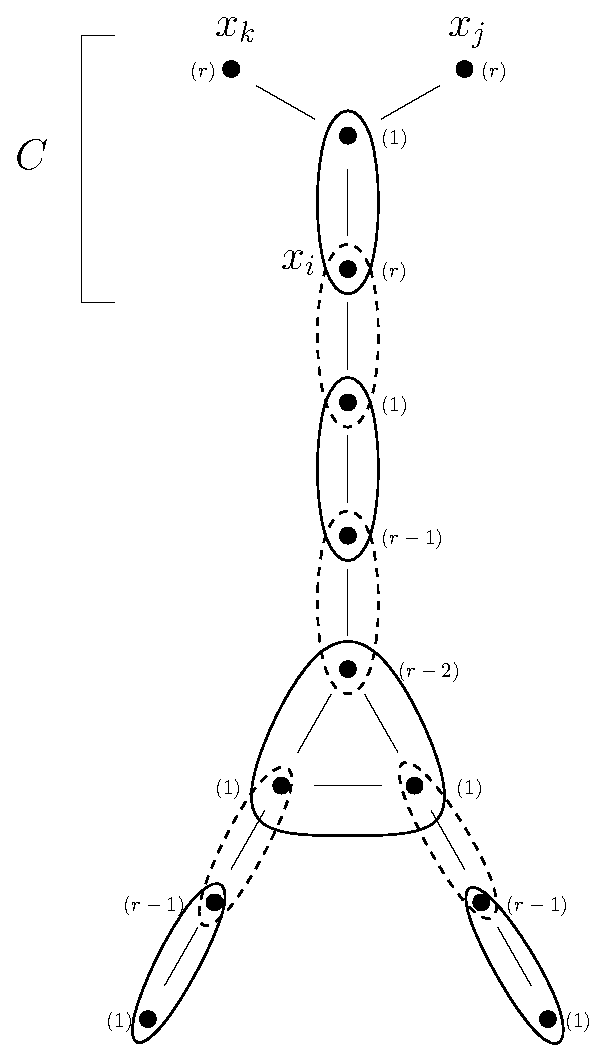
\includegraphics[scale=.6]{figs/hardness}
\caption{clause and splitter gadget}
\label{fig:3satconstruction}
\end{center}
\end{figure}

\begin{figure}[htbp]
\begin{center}
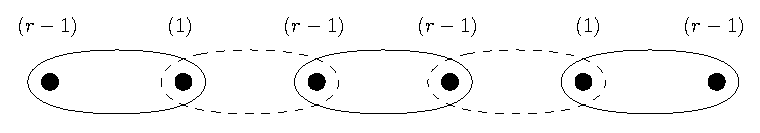
\includegraphics[scale=.8]{figs/negation}
\caption{signal negation gadget}
\label{fig:negation}
\end{center}
\end{figure}

\begin{theorem}
The r-gather problem for the case where the diameter of a cluster is measured by the diameter of the smallest covering disk is NP-hard to approximate better than a factor of ${\sqrt{35}+\sqrt{3} \over 4} \approx 1.912$ when $r\geq4$.
\end{theorem}
\begin{proof}
The reduction is very simlar to the proof of Theorem~\ref{thm:hardness1}.  The only difference is the splitter which is illustrated in Figure~\ref{fig:splitter}.
\end{proof}

\begin{figure}[htbp]
\begin{center}
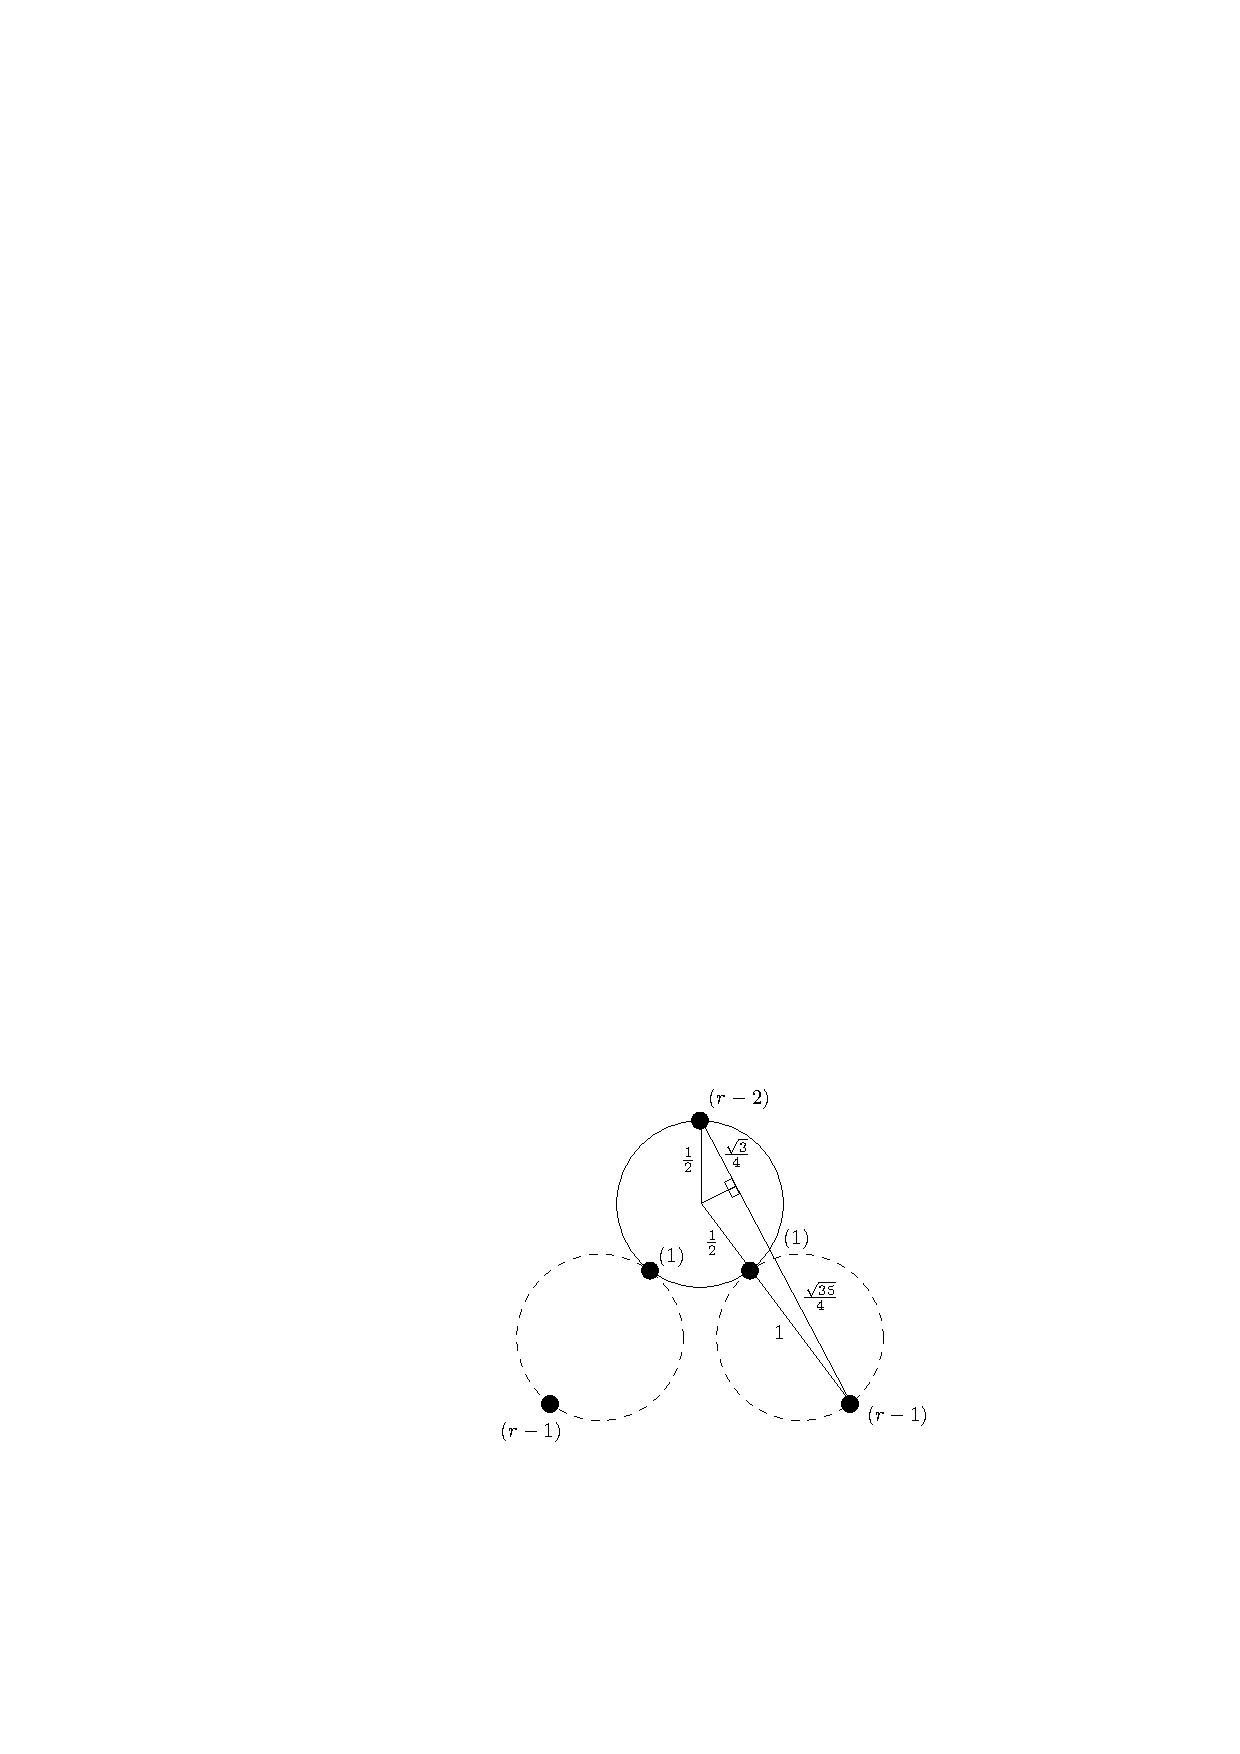
\includegraphics[scale=.9]{figs/splitter}
\caption{close up of the splitter}
\label{fig:splitter}
\end{center}
\end{figure}

\begin{theorem}
The r-gather problem for the case where the diamter of a cluster is measured by the diameter of the smallest covering disk is NP-hard to approximate better than a factor of $\sqrt{13}/2 \approx 1.802$ when $r=3$.
\end{theorem}
\begin{proof}
We reduce from the NP-hard problem planar circuit SAT.  We are given a planar boolean circuit with a single output.  Similar to the previous proofs, a wire gadget consists of a line of points that alternate between a single point and a group of $r-1$ points at the same location.  The parity of the clusters chosen signify a true signal or a false signal.  When the clusters combine a group of $r-1$ points followed by a single point, the signal of the wire is true.  It is simple to enforce the output to be a true signal by ending the output wire with a single point.  The beginning of the input wires have a group of $r$ points so that the inputs can be either true or false.  Figure~\ref{fig:nandgadget} illustrates the NAND gadget, a universal gate.  The solid clusters illustrate two true inputs into the gate and a false output.  If either or both of the inputs is false, then two groups of points in the triangle (or all three) will become a cluster and the output will be true.  Figure~\ref{fig:splittercircuit} ilustrates the splitter circuit where the solid clusters indicate a true signal and the dashed clusters indicate a false signal.  As before, if the optimal solution to the $r$-gather construction can be found, then cluster diameter will be 1.  Otherwise, three groups will form a cluster, two from the triangle and one adjacent to the triangle.  The diameter of such a cluster is $\sqrt{13}/2 \approx 1.802$ when $r=3$.  Finally, note that in order to connect the wires, they must be able to turn somehow.   We can bend the wire such that no three groups of points can form a cluster that has diameter smaller than $\sqrt{13}/2$.  Thus concludes our proof.
\end{proof}

\begin{figure}[htbp]
\begin{center}
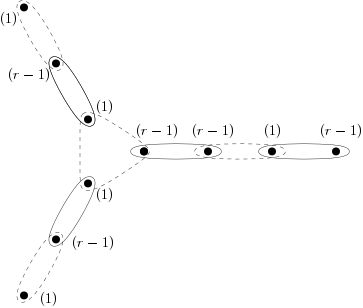
\includegraphics[scale=.6]{figs/nandgadget}
\caption{NAND gadget}
\label{fig:nandgadget}
\end{center}
\end{figure}

\begin{figure}[htbp]
\begin{center}
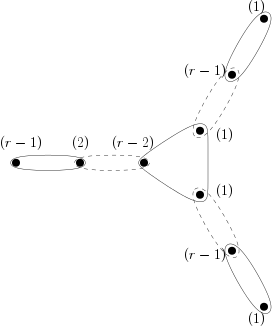
\includegraphics[scale=.6]{figs/splittergadget}
\caption{splitter gadget}
\label{fig:splittercircuit}
\end{center}
\end{figure}

\begin{theorem}
The r-gather problem for the case where the diameter of a cluster is the distance between the furthest pair of points is NP-hard to approximate better than $\sqrt{2+\sqrt{3}} \approx 1.931$ when $r=3$ or $4$.
\end{theorem}

\section{Dynamic $r$-Gather}

The natural progression of investigating the $r$-gather problem is to consider clustering when the points are mobile.  The conversion of the $r$-gather problem to a dynamic setting may appear in many forms.  In this section, we detail several versions of the mobile $r$-gather problem.  In each version, we assume that the trajectories of the points are piecewise linear.

In the simplest formulation of $r$-gather in a mobile setting, we are given a set of trajectories over a time period $T$ and we want to cluster the trajectories such that each cluster has at least $r$ trajectories and the largest diamteter of each cluster over the entire time period is minimized.  Here we designate the diameter of a cluster at a single point in time to be the distance between the furthest pair of points.  Points are assigned to a single cluster for the entire length of $T$ and do not switch clusters.  We claim that the 2-approximation strategy for static $r$-gather can also be applied to this problem.  
%We also claim that 2-inapproximation lower bound from Aggarwal et. al. applies as well \cite{Aggarwal06achievinganonymity}.  
We use the distance metric defined by Lemma~\ref{lem:distancemetric}.  

\begin{lemma}\label{lem:distancemetric}
The distance function $d_t(p,q)$ between two trajectories $p$ and $q$ over a time period $T$ is defined as the distance between $p$ and $q$ at time $t \in T$.  Then $d(p,q) = \max_{t \in T}d_t(p,q)$.  The function $d(p,q)$ is a metric.
\end{lemma}

\begin{proof}
The function by definition is symmetric, follows the identity condition, and is always non-negative.  To show that the metric follows the triangle equality, we first assume that there is a pair of trajectories $x$ and $z$ where $d(x,z) > d(x,y) + d(y,z)$ for some $y$.  There is some time $t \in T$, where $d_t(x,z) = d(x,z)$.  By triangle inequality,
$$d_t(x,z) \leq d_t(x,y) + d_t(y,z).$$
This contradicts our assumption and concludes our proof.
\end{proof}

%\begin{theorem}
%For the definition of dynamic $r$-gather where all trajectories are clustered once, it is NP-hard to approximate better than a factor of 2 for $r > 6$.
%\end{theorem}

%\begin{proof}
%We construct a reduction from the problem 3-SAT where each variable is restricted to 3 clauses.  Our proof is similar to the lower bound proof in \cite{Aggarwal06achievinganonymity}.  Given a boolean formula in 3-CNF form with $m$ clauses $C_j$, $1 \leq j \leq m$, composed of $n$ variables $x_i$, $1 \leq i \leq n$, where $i$ and $j$ are integers, we construct a set of trajectories over a time period $T$.  For every variable $x_i$ and its complement $\bar{x_i}$, we have two points $v_i^T$ and $v_i^F$ and an additional $(r-2)$ points $u_i^k$ for integer $k$, $1 \leq k \leq r-2$.  We will construct trajectories where $d(v_i^T, v_i^F) = d(v_i^T, u_i^k) = d(v_i^F, u_i^k) = 1$, for $1 \leq i \leq n$ and $1 \leq k \leq r-2$ .  In addition, for every cluster $C_j$, we construct another point $w_j$.  We construct trajectories such that the distance between $w_j$ and the points that represent the literals in the clause $C_j$ is 1.  All other distances are 2.

%Constructing the trajectories that obey these distance constraints is simple.  Place all points at the origin on a number line.  For every point $p$, we have one timestep that establishes the distance between it and all other points.  In that timestep, $p$ moves to 2 on the number line.  At the same time, all other points that must have a distance of 1 to $p$ move to 1 on the number line.  This procedure is repeated for every point.

%We claim, that if there is an $r$-gather clustering of maximum radius 1, then the 3-SAT formula can be satisfied.  Here, for every variable, we have two possibilities for the center of a cluster of radius 1, $v_i^T$ and $v_i^F$.  There are not enough points close to $v_i^T$ and $v_i^F$ to have both as the center of two clusters.  Any cluster with $u_i^k$ as the center will have fewer than $r$ points within a distance of 1 and therefore cannot be a cluster center with radius 1.  Finally, every point $w_j$ has only three other points within a distance of 1.  Therefore, in any $r$-gather clustering with maximum radius 1, there is one cluster for every variable with a center of either $v_i^T$ or $v_i^F$.  This clustering must be done in such a way that for every point $w_j$, at least one of the points that represents a literal in $C_j$ must be chosen as a cluster center.  Thus if an optimal $r$-gather clustering of our trajectories can be found, then we can determine if the corresponding 3-SAT formula is satisfiable.
%\end{proof}

The next step in expanding dynamic $r$-gather is by allowing the clusters to change throughout $T$.  We amend our problem formulation to allow $k$ regroupings.  Each regrouping allows all clusters to be modified or changed completely.  The lower bounds for the earlier version of $r$-gather applies here too for the same reasons.  We claim that with the assumption that the trajectories are piecewise linear, we can construct a 2-approximation solution using dynamic programming.

Let $|T|$ be the number of timesteps in the time period $T$.  Each trajectory is a piecewise linear function that only changes directions at a timestep in $T$.  Let $C_{ij}$ denote the max diameter of the 2-approximation clustering at time $i$ over the time period $[i,j]$, $i<j$.  We can create a $|T| \times |T|$ table $\mathcal{T}$ where entry $\mathcal{T}(i, j) = C_{ij}$.  One clustering takes $O(\frac{1}{\epsilon}kn^2)$ and there are $|T|$ clusterings in total.  However, for each clustering, the max diamter is recalculated for each timestep.  The cost of recalculating the max diameter of a clustering is $O(n/r)$.  The total number of times a clustering is recalculated is $O(n|T|/r)$.  The total time it takes to compute the table $\mathcal{T}$ is $O(n|T|^2/r + \frac{1}{\epsilon}k|T|n^2)$.

We formulate a subproblem $S(t,i)$, where $0 \leq t \leq |T|$ and $i \leq k$, for our dynamic program to find the optimal clustering of the points in the time period $[0, t]$ where there are exactly $i$ reclusterings.  Let $l(t,i)$ denote the last timestep a reclustering occured for the optimal solution of $S(t,i)$.

The subproblem of our dynamic program is:

$$S(t,i) = \min( \max_{j<t}(S(j, i), C_{l(t,i)t}), \max_{j<t}(S(j, i-1), C_{tt}) )$$ 

The entry $S(t,i)$ checks $2t$ previous entries and $2t$ entries in the table $\mathcal{T}$.  The entire table takes $k|T|^2$ to execute with the additional preprocessing of the table $\mathcal{T}$.

Our lower bound proofs for static $r$-gather apply here as well.  The points arranged in any of the lower bound proofs can be static points for the duration of $T$ or may move in a fashion where the 
distances between points do not increase.  Then the arguments for static $r$-gather translate to this simple version of dynamic $r$-gather directly.

\begin{theorem}
The lower bound results for static $r$-gather apply to any definition of dynamic $r$-gather.  Further, we can approximate mobile $r$-gather, when $k$ clustergings are allowed, within a factor of 2.
\end{theorem}

Another variation allows unlimited regroupings in a continuous dynamic setting.  We know that in this setting, the optimal clustering may change many times, as much as $O(n^3)$ times.  Consider this example: $n/2$ points lie on a line where the points are spaced apart by 1 and 3 points are overlapping on the ends.  In this example, $r = 3$.  The optimal clustering of the points on the line is to have three points in a row be in one cluster with a diameter of $2$.  There are three different such clusterings which differ in the parity of the clusterings.  In each clustering, there are $O(n)$ clusters.  If another point travels along the line, when it is within the boundaries of a cluster, it will just join that cluster.  However, when it reaches the boundary of a cluster and exits it, the optimal clustering would be to shift the parity of the clustering.  This results in a change in all of the clusters along the line.  The clustering change every time the point travels a distance of 2.  Therefore, as the point travels along the line, the number of times the entire clustering changes is $O(n)$ which results in a total of $O(n^2)$ changes to individial clusters.  Since there are $O(n)$ points that travel along the line, the total number of clusters that change is $O(n^3)$.

\section{Decentralized $r$-Gather}

In this section, we describe a 4-approximation algorithm for $r$-gather that is less centralized than the 2-approximation in \cite{Aggarwal06achievinganonymity}.  We begin with an algorithm that is not explicitly decentralized and then later detail how to do so.

Let the $r$-neighborhood of a point $p_i$ or $N_r(p_i)$ denote the set containing $p_i$ and the closest $r-1$ points to $p_i$.  Let $N$ be the set of the $r$-neighborhoods of all points in $P$.  For each $r$-neighborhood, we define a distance $R_i^r = \max_{p_j \in N_r(p_i)}||p_i - p_j||$ and we define a distance $R^r = \max_{1 \leq i \leq n}R_i^r$ among all $r$-neighborhoods.  We first find a maximal independent set $S$ of $r$-neighborhoods.  For an $r$-neighborhood $N_r(p_i)$, we name $p_i$ the center of the cluster and all other points in $N_r(p_i)$ are named the cannonical set.  Each point $p_i$ that is not in a set in $S$ must have at least one point in it's $r$-neighborhood that is in a set in $S$ (otherwise $S$ is not maximal).  We assign $p_i$ to the set of one of these points.  Such a point is named an outer member of its set.  We claim that the resulting clustering $S'$ is a 4-approximation $r$-gather clustering.  

\begin{theorem}
This algorithm is a 4-approximation.
\end{theorem}

\begin{proof}
Let $d_{OPT}$ be the diameter of the largest cluster of the optimal $r$-gather clustering.  We claim that any cluster containing a point and $r-1$ other points must have a diameter greater than or equal to $R^r$ and therefore $R^r \leq d_{OPT}$.  Wlog, let $N_r(p_i) \in S$.  We define the corresponding cluster in $S'$ to be $s_i$.  A cluster $s_i$ in $S'$ is made up of the $r$-neighborhood of $p_i$ and points whose $r$-neighborhood intersect with $N_r(p_i)$.  Let $p_j$ be one of the latter points.  The distance between $p_j$ and any point in $N_r(p_j) \cap N_r(p_i)$ is no greater than $R^r$.  By definition, $R^r \geq R_i^r$.  By triangle inequality, no point in $s_i$ is further than $2R^r$ from $p_i$.  Therefore, the diameter of any cluster in $S'$ cannot be greater than $4R^r \leq 4d_{OPT}$.
\end{proof}

To decentralize this algorithm, we only need to find a maximal independent set of $r$-neighborhoods in a decentralized fashion.  This may include a randomized solution for maximal independent set or a distributed, deterministic algorithm for finding local maximums.

Such a clustering can be maintained while the points move.  Every point must keep track of its $r$-neighborhood.  Critical events, events when clusterings may change, occur when a point's $r$-neighborhood changes or when its is released from its current cluster.  To maintain a $4$-approximation clustering, when a critical event happens, the nodes must behave as the following.

When a point's, $p_i's$, $r$-neighborhood changes, if the point is:
\begin{enumerate}
\item A center of a cluster - if the new member of $p_i's$ $r$-neighborhood is:
\begin{enumerate}
\item A center or cannonical member of another cluster - then $p_i$ becomes an outer member of the other point's cluster, all other points in $p_i's$ previous cluster are released from the cluster.
\item An outer member of another cluster - the other point becomes a cannonical member of $p_i's$ cluster
\end{enumerate}
\item A member of a cannonical set or an outer member of a set - do nothing
\end{enumerate}

When a point, $p_i$, has been released from a cluster, if the point is:
\begin{enumerate}
\item A center of a cluster - doesn't happen
\item A member of a cannonical set or an outer member
\begin{enumerate}
\item if its $r$-neighborhood contains a center or cannonical member of another set - $p_i$ joins that cluster as an outer member
\item otherwise - $p_i$ and it's $r$-neighborhood can form it's own cluster
\end{enumerate}
\end{enumerate}

\section{Acknowledgements}
This project was supported by NSF grant CCF-1017539.

\begin{small}
\bibliographystyle{abbrv}
\bibliography{r-gather}
\end{small}
\end{document}